% !TeX spellcheck = en_US
%-----------------------------------------------------------------------
%
%\documentclass[referee]{aa} % for a referee version
%\documentclass[onecolumn]{aa} % for a paper on 1 column
%\documentclass[longauth]{aa} % for the long lists of affiliations
%\documentclass[letter]{aa} % for the letters
%\documentclass[bibyear]{aa} % if the references are not structured
%                              according to the author-year natbib style

\documentclass{aa}

\usepackage[utf8]{inputenc}
\usepackage[T1]{fontenc}
\usepackage{txfonts}
%\usepackage{bbm}
%\usepackage{dsfont}
%\usepackage{textcomp}
%\usepackage{mathrsfs}
\usepackage{stmaryrd}

%\newcommand*{\PDFTitle}{Calibration of scientific image detectors}
%\newcommand*{\PDFAuthors}{É.\ Thiébaut et al.}

\DeclareUnicodeCharacter{00B5}{\ensuremath{\mu}} % µ
\DeclareUnicodeCharacter{2264}{\ensuremath{\le}} % ≤
\DeclareUnicodeCharacter{2265}{\ensuremath{\ge}} % ≥
\DeclareUnicodeCharacter{22C5}{\ensuremath{\!\cdot\!}}

\newcommand{\Hide}[1]{}
\newcommand{\Show}[1]{#1}

\usepackage{amsmath,amsfonts,amssymb}
%\usepackage{amsthm}
\usepackage{mathtools}

%\usepackage[authoryear,round,semicolon]{natbib}

\usepackage[squaren,Gray]{SIunits}
\usepackage{xspace}

\usepackage[ruled,vlined]{algorithm2e}
\usepackage{algpseudocode}

\usepackage{graphicx}
\graphicspath{{figs/}}

\usepackage[x11names,hyperref]{xcolor}
\newcommand{\oops}[1]{\textcolor[named]{OrangeRed1}{#1}}

\usepackage[unicode=true, colorlinks=true, linkcolor=Purple2, urlcolor=Purple2,
citecolor=Purple4]{hyperref}

%\usepackage[unicode=true,
% bookmarks=true,bookmarksnumbered=false,bookmarksopen=false,
% breaklinks=true,pdfborder={0 0 0},backref=page,colorlinks=true]{hyperref}
%\hypersetup{
%  pdftitle={\PDFTitle},
%  pdfauthor={\PDFAuthors},
%  unicode=true,
%  linkcolor=Purple1,
%  urlcolor=Purple1,
%  citecolor=Purple1,
%  filecolor=Purple1,
%  menucolor=Purple1,
%  pagecolor=Purple1}

\newcommand{\newstuff}[1]{{\color{magenta}#1}}
\newcommand{\strong}[1]{\textbf{\emph{#1}}}
\newcommand*{\code}[1]{\texttt{#1}}
\newcommand*{\variable}[1]{\texttt{#1}}
\newcommand*{\FileName}[1]{\texttt{#1}}

% Abbreviations:
\newcommand*{\etal}{\emph{et al.}\xspace}
\newcommand*{\etc}{\emph{etc.}\xspace}
\newcommand*{\eg}{\emph{e.g.}\xspace}
\newcommand*{\ie}{\emph{i.e.}\xspace}

%%%%%%%%%%%%%%%%%%%%%%%%%%%%%%%%%%%%%%%%%%%%%%%%%%%%%%%%%%%%%%%%%%%%%%%%%%%%%%%%
%\useosf % no longer required if osf specified, otherwise after all math
\DeclareSymbolFont{bbold}{U}{bbold}{m}{n}
\DeclareSymbolFontAlphabet{\mathbbold}{bbold}
\RequirePackage{textcomp}  % required for special glyphs

% Parenthesis:
%\def\Paren{}\let\Paren\undefined
\DeclarePairedDelimiterX{\Paren}[1]{(}{)}{#1}
\DeclarePairedDelimiterX{\Brace}[1]{\{}{\}}{#1}
\DeclarePairedDelimiterX{\Brack}[1]{[}{]}{#1}
\DeclarePairedDelimiterX{\Abs}[1]{\rvert}{\lvert}{#1}
\DeclarePairedDelimiterX{\Norm}[1]{\lVert}{\rVert}{#1}
\DeclarePairedDelimiterX{\Group}[1]{\lgroup}{\rgroup}{#1}
%\DeclarePairedDelimiterX{\FrobNorm}[1]{\lVert}{\rVert_{\Tag{F}}}{#1}
\DeclarePairedDelimiterX{\Avg}[1]{\langle}{\rangle}{#1}
\DeclarePairedDelimiterX{\Round}[1]{\lfloor}{\rceil}{#1}
\DeclarePairedDelimiterX{\Floor}[1]{\lfloor}{\rfloor}{#1}
\DeclarePairedDelimiterX{\Ceil}[1]{\lceil}{\rceil}{#1}
%\DeclarePairedDelimiterX{\Inner}[2]{\langle}{\rangle}{#1\,\delimsize\vert\,#2}
\DeclarePairedDelimiterX{\Inner}[2]{\langle}{\rangle}{#1,#2}
%\DeclarePairedDelimiterXPP{\IndexedList}[3]{}\{\}{_{#2}^{#3}}{#1}
\DeclarePairedDelimiterXPP{\IndexedList}[3]{}\{\}{_{#2,\ldots,#3}}{#1}
\DeclarePairedDelimiterX{\IntRange}[1]{\llbracket}{\rrbracket}{#1}

% A list \List{ELEM}{START}{END}
\DeclarePairedDelimiterXPP{\List}[3]{}{\{}{\}}{_{#2,\ldots,#3}}{#1}

\newcommand*{\delimsize}{}
\newcommand*{\suchthat}{\,\vert\,} % compact version
\newcommand*{\SuchThat}{\:\delimsize\vert\:} % autoscale to surrounding version
\newcommand*{\given}{\,\vert\,} % compact version
\newcommand*{\Given}{\:\delimsize\vert\:} % autoscale to surrounding version
%\newcommand*{\given}{\mathbin{\vert}}
%\newcommand*{\Given}{\mathrel{\delimsize\vert}} % autoscale to surrounding
%%version

% Upright letters:
\newcommand*{\mathd}{\mathrm{d}}
\newcommand*{\mathe}{\mathrm{e}}
\newcommand*{\mathi}{\mathrm{i}}

% Operators/functions
\renewcommand*{\Re}{\operatorname{Re}}
\renewcommand*{\Im}{\operatorname{Im}}
\DeclareMathOperator*{\argmin}{arg\,min}
\DeclareMathOperator*{\argmax}{arg\,max}
\DeclareMathOperator{\arc}{arc}
\DeclareMathOperator{\rnd}{rnd}
\DeclareMathOperator{\sign}{sign}
\DeclareMathOperator{\sinc}{sinc}
\DeclareMathOperator{\Card}{Card}
\DeclareMathOperator{\Conv}{conv}
%\DeclareMathOperator{\Det}{Det}
\newcommand*{\Det}{\det}
\DeclareMathOperator{\Diag}{diag}
\DeclareMathOperator{\Dom}{dom}
\DeclareMathOperator{\Prox}{prox}
\DeclareMathOperator{\Rank}{rank}
\DeclareMathOperator{\Sign}{sign}
\DeclareMathOperator{\Span}{span}
\DeclareMathOperator{\Trace}{tr}
\newcommand*{\trace}{\Trace}

% Statistics:
%\DeclareMathOperator{\Var}{Var}
%\DeclareMathOperator{\Cov}{Cov}
%\DeclareMathOperator{\Expect}{E}
%\newcommand*{\Expect}{\mathbb{E}}
\DeclarePairedDelimiterXPP{\Var}[1]{\mathrm{Var}}(){}{#1}
\DeclarePairedDelimiterXPP{\Cov}[1]{\mathrm{Cov}}(){}{#1}
\DeclarePairedDelimiterXPP{\Expect}[1]{\mathrm{E}}(){}{#1}
\DeclarePairedDelimiterXPP{\LogPr}[1]{\ell}(){}{#1}

% Sets:
\newcommand*{\Set}[1]{\mathbb{#1}}
\newcommand*{\Reals}{\Set{R}}
\newcommand*{\Integers}{\Set{Z}}
\newcommand*{\NaturalNumbers}{\Set{N}}
\newcommand*{\Rationals}{\Set{Q}}
\newcommand*{\Complexes}{\Set{C}}

% Miscellaneous:
\newcommand*{\Tag}[1]{\mathsf{#1}}
\newcommand*{\PDer}[2]{\frac{\partial#1}{\partial#2}}
\newcommand*{\bydef}{\stackrel{{\scriptscriptstyle \text{def}}}{=}}
\newcommand*{\TwoIPi}{2\,\mathi\,\pi}
%\newcommand*{\rand}[1]{\widetilde{#1}} % random value/variable
%\newcommand*{\rand}[1]{\tilde{#1}} % random value/variable
%\newcommand*{\SIM}{\text{\raisebox{-0.3ex}[0pt][0pt]{$\sim$}}}
\newcommand*{\SIM}{\smash{\sim}}
\newcommand*{\proxy}[1]{\overset{\SIM}{#1}} % random value/variable
%\newcommand*{\proxy}[1]{\widetilde{#1}}
\newcommand*{\estim}[1]{\hat{#1}}
%\newcommand*{\estim}[1]{\widehat{#1}}
%\newcommand*{\FT}[1]{\widehat{#1}}
%\newcommand*{\FT}[1]{\mathring{#1}}
\newcommand*{\FT}[1]{\widetilde{#1}}
\newcommand*{\MathNote}[2]{\hspace*{#1}\text{\footnotesize(#2)}}
\newcommand*{\better}[1]{#1^{+}}
\newcommand*{\best}[1]{#1^{\star}}
\newcommand*{\Combine}{{\circ}}
\newcommand*{\EndProof}{\blacksquare}


% ========== LINEAR ALGEBRA ==========

\newcommand*{\V}[1]{\boldsymbol{#1}}   % a vector
\newcommand*{\M}[1]{\mathbf{#1}}       % an operator (a matrix)

%\newcommand*{\TransposeLetter}{\top}
\newcommand*{\TransposeLetter}{\mathrm{t}}
\newcommand*{\T}{^{\TransposeLetter}}
\newcommand*{\mT}{^{-\TransposeLetter}}

% The following definition is to remove surrounding spacing around ⋅
% to denote dot product.
\newcommand*{\MDot}{\mathord{\,\mathchar"2201\,}}
\newcommand*{\Tcdot}{\T\!⋅}

\newcommand*{\QuadTerm}[2]{#2\T\MDot#1\MDot#2}
\newcommand{\ArrayWithDelimiters}[4]{%
  \left #1\begin{array}{#2}#4\end{array}\right #3}
\newcommand{\Matrix}[2]{\ArrayWithDelimiters{\lgroup}{#1}{\rgroup}{#2}}
\newcommand{\Vector}[1]{\ArrayWithDelimiters{\lgroup}{c}{\rgroup}{#1}}
\newcommand{\TwoByTwoMatrix}[4]{\Matrix{cc}{#1 & #2 \\ #3 & #4 \\}}
\newcommand{\TwoByTwoSymmetricMatrix}[3]{\TwoByTwoMatrix{#1}{#3}{#3}{#2}}

\newcommand*{\textfrac}[2]{\ensuremath{\textstyle\frac{#1}{#2}}}
\newcommand*{\scriptfrac}[2]{\ensuremath{\scriptstyle\frac{#1}{#2}}}

%\newcommand*{\One}{1\hspace*{-0.8ex}1}
%\newcommand*{\Zero}{0\hspace*{-0.8ex}0}
%\newcommand*{\One}{\mathbbm{1}}
%\newcommand*{\Zero}{\mathbbm{0}}
\newcommand*{\One}{\mathds{1}}
\newcommand*{\Zero}{\mathds{O}}
%\newcommand*{\Zero}{\V 0}
%\newcommand*{\One}{\V 1}

% Macros to add a bit of spacing around text in equations.
%    \TextSpace     = insert some amount of spacing
%    \MidText{text} = insert text in the middle of equations
%    \EndText{text} = insert text at the end of an equation
%    \BegText{text} = insert text at the beginning of an equation
\newcommand*{\TextSpace}{\mspace{12mu}}
\newcommand*{\MidText}[1]{\TextSpace\text{#1}\TextSpace}
\newcommand*{\EndText}[1]{\TextSpace\text{#1}}
\newcommand*{\BegText}[1]{\text{#1}\TextSpace}

%------------------------------------------------------------------------------
% Ref: Alexander R. Perlis., "A complement to \smash, \llap, and \rlap,"
%      TUGboat, Vol. 22, pp. 350-352, 2001.
%      <http://math.arizona.edu/~aprl/publications/mathclap/>
%
% For comparison, the existing overlap macros:
% \def\llap#1{\hbox to 0pt{\hss#1}}
% \def\rlap#1{\hbox to 0pt{#1\hss}}
  \def\clap#1{\hbox to 0pt{\hss#1\hss}}
  \def\mathllap{\mathpalette\mathllapinternal}
  \def\mathrlap{\mathpalette\mathrlapinternal}
  \def\mathclap{\mathpalette\mathclapinternal}
  \def\mathllapinternal#1#2{\llap{$\mathsurround=0pt#1{#2}$}}
  \def\mathrlapinternal#1#2{\rlap{$\mathsurround=0pt#1{#2}$}}
  \def\mathclapinternal#1#2{\clap{$\mathsurround=0pt#1{#2}$}}

%----------------------------------------------------------[SIMPLE ALGORITHMS]-

\newcommand{\CodeBlock}[1]{\begin{array}{l}#1\end{array}}
\newcommand{\FloorBlock}[1]{\left\lfloor\CodeBlock{#1}\right.}
\newcommand{\VertBlock}[1]{\left\lvert\CodeBlock{#1}\right.}

%------------------------------------------------------------------[NOTATIONS]-

\newcommand*{\SampleTag}{\Tag{smp}}
\newcommand*{\Samples}{{N_\SampleTag}}
\newcommand*{\Pixels}{{N_\Tag{pix}}}
\newcommand*{\Images}{{N_\Tag{img}}}
\newcommand*{\Dimensions}{{N_\Tag{dim}}}
\newcommand*{\Cost}{\mathcal{J}}
\newcommand*{\Correl}{\mathcal{C}}
%\newcommand*{\Filtered}[1]{\widetilde{#1}}
\newcommand*{\Filtered}[1]{\mathring{#1}}
\newcommand*{\Approx}[1]{\widetilde{#1}}
\newcommand*{\noise}{n}
\newcommand*{\Iter}[1]{^{[#1]}}

% ADU and electrons are not really units but it is useful to define them
% as such.
%\newcommand{\electron}{{\text{e}^-}}
\addunit{\electron}{e^-}
\addunit{\ADU}{ADU}

\begin{document}


\title{Calibration of scientific image detectors}

%\subtitle{A global approach for calibrating scientific image detectors}

\author{
  Éric Thiébaut\inst{1}
  \and Michel Tallon\inst{1}
  \and Samuel Thé\inst{1}
  \and Laurence Denneulin\inst{1}
  \and Ferréol Soulez\inst{1}
  \and Anthony Berdeu\inst{1,2}
}

\institute{
  CRAL\\
  \email{eric.thiebaut@univ-lyon1.fr}
  \and
  NARIT
}

\date{Received xxx; accepted xxx}

\abstract
% context heading (optional)
% {} leave it empty if necessary
{Image detectors are widely used in astronomy for instruments that are more
and more complex requiring elaborated post-processing methods to extract
information of interest.}
% aims heading (mandatory)
{The purpose of this paper is to present a flexible method to extract relevant
calibration parameters for pre-processing detector data so as to provide
sufficient statistics.}
% methods heading (mandatory)
{Methods.}
% results heading (mandatory)
{Results.}
% conclusions heading (optional), leave it empty if necessary
{Conclusions.}

\keywords{detector -- }

 \maketitle
%
%-------------------------------------------------------------------

\section{Introduction}

For any serious imaging application based on empirical data, proper calibration
of the detector is necessary to obtain an unbiased estimator of the light level
seen by each pixel and the corresponding variance or precision.


\oops{See \citet{Foi_et_al-2008-Poissonian_Gaussian_noise_model_fitting}}

Note: other approaches for considering non-uniform noise level: Anscombe
transform, exact Guassian + Poissonian PDF, pragmatic models (like the
proposed Gaussian approximation).


The paper is organized as follows. We first show that accounting for the analog
to digital converter yields subtle digitization effects that rule out the most
elaborate statistics developed to describe the data delivered by a detector.
We therefore advocate that a simple non-homogeneous Gaussian approximation is a
good enough approximation. We then propose a global approach to jointly fit the
pixelwise parameters of the detector model on all relevant calibration data.




\section{Modeling the detector}
\label{sec:detector-model}

We consider imaging at optical wavelengths (visible or infrared) with a CMOS or
a CCD device.


\subsection{Principle of photon detection}
\label{sec:detection-principle}

Light detection is based on the photo-electric effect that occurs in the
metal-oxide-semiconductor of which the sensor is made. The photo-electric effect
converts a photon into an electron which is captured by the well of the pixel.
For each incident photon, the probability of success of this process is called
the \emph{quantum efficiency} of the pixel.  During the exposure, thermal
jittering of the electrons in the substrate may cause some electrons to overcome
the potential barrier of the well and be captured.  The number of such captured
thermal electrons grows linearly with the time\footnote{provided the amount of
captured electrons is negligible compared to the total number of electrons in
the substrate and the full-well capacity is not exceeded}, hence the name of
\emph{dark current} for this contribution to the signal. During the reading, the
number of captured electrons is converted to a digital number in so-called
\emph{Analog-Digital Units} (ADU), usually an integer encoded in a given number
of bits.  The counting of the number of electrons is not perfect and introduces
so called \emph{readout-out} noise, besides, the conversion in ADUs introduces
rounding errors and have an incidence on their statistics as we show next.

\oops{[ET: Summarize other possible sources of errors: the readout noise, the
cross-talk between close pixels, electrons loss/gain during the charge transfer
for charge coupled devices (CCD), or electron multiplying CCD (EMCCD), \etc]}

\oops{[ET: Another important assumption made later is that errors are mutually
independent between pixels.]}


\subsection{Effects of digitization}
\label{sec:digitization}

The number $n_{\electron}$ of electrons transferred\footnote{$n_{\electron}$
accounts for the photo-electrons that are captured by the pixel well but also
for the electrons contributed by the \emph{dark current}; in what follows, the
electrons gained or lost during the transfer are assumed to be part of the
readout noise} by a given pixel to the analog to digital converter (ADC) is is
a random variable having a Poisson distribution of parameter $\mu =
\Expect{n_\electron}$ the mean number of electrons, $\Expect{\ldots}$ denoting
the expectation.  The randomness of $n_\electron$ is called the \emph{shot
noise} and, as explained before, is not the only source of noise or errors in
the values given by a detector.  To simplify the discussion, we call
\emph{readout noise} all random perturbations other than the shot noise.

To account for the various sources of noise, the digitized value may be assumed
to be given by:
\begin{equation}
  d = \Round*{(n_{\electron}/g) + z + \omega} \, ,
  \label{eq:ADC-model}
\end{equation}
where $z$ is the \emph{zero-level} (also called \emph{bias}) of the ADC, $g$ is
the \emph{gain} of the ADC, $\omega$ is a random variable accounting for the
readout noise and $\Round{\ldots}$ denotes conversion to an integer number of
ADUs.  The zero-level $z$ and the readout noise $\omega$ are expressed in ADUs
while the gain $g$ is in electrons per ADU ($\electron/\ADU$).

In Eq.~\eqref{eq:ADC-model}, $\Round{x} \in \Integers$ denotes the conversion
of the input value $x \in \Reals$ to some integer output value. Typically,
$\Round{x}$ rounds its argument to the nearest integer\footnote{a different
assumption is equivalent to changing the zero-level $z$} within some limits:
\begin{equation}
  \Round{x} = \min\Paren*{
    \max\Paren*{
      \Floor*{x + \textfrac12}, d_\Tag{min}
    }, d_\Tag{max}
  }
  \label{eq:digitization}
\end{equation}
with $\Floor{\ldots}$ the floor function and with $d_\Tag{min}$ and
$d_\Tag{max}$ the minimum and maximum output levels of the converter. Usually,
the clipping limits are $d_\Tag{min} = 0$ and $d_\Tag{max} = 2^{n_\Tag{bits}} -
1$ with $n_\Tag{bits}$ the number of bits encoding the output value. Note that
the upper clipping bound $d_\Tag{max}$ is not the same thing as the saturation
phenomenon which is due to the finite full-well capacity of the considered
pixel.  In what follows, we will focus on the consequences of the rounding
errors caused by the conversion to an integer and assume that clipping of
values does not occur. In the processing of the data, this amounts to imposing
that saturated pixels (whatever the reason) be considered as defective and
discarded.

The zero-level $z$ can take into account any constant bias so, without loss of
generality, we can assume that the readout noise is centered, \ie that
$\Expect{\omega} = 0$. \citet{Winick-1986-Cramer_Rao} assumes that the readout
noise be Poissonian as is the number $n_\electron$ of electrons so that, in
photon counting mode, the distribution of ADUs is Poissonian (and biased).  In
our model in Eq.~\eqref{eq:ADC-model}, photon counting mode would correspond to
having $g=1$ and $z \in \Integers$.  Actual photon counting detectors however
involve light intensification (in ICCD, for \emph{Intensified CCD}) or electron
multiplication (in EMCCD) and their output can have very different statistics
\citep[\eg,][]{Thiebaut-1994-photon_counting_speckle_interferometry}.  Such
detectors are out of the scope of the present paper. Most other authors
\citep[\eg,][\etc]{Murtagh_et_all-1995-multiresolution,
Foi_et_al-2008-Poissonian_Gaussian_noise_model_fitting,
Chouzenoux_etal-2015-exact-Poisson_Gaussian_likelihood,
Boulanger_etal-2018-nonsmooth_convex_optimization} assume that the readout
noise $\omega$ be Gaussian but do not consider digitization effects and model
the
statistics of the ADUs as a mixture of Poisson and Gaussian noises. As shown
next, the unavoidable digitization introduces rounding errors which rule out
modeling the ADUs statistics as an \emph{exact} mixture of Poisson and Gaussian
noises.

\begin{figure}
\centering
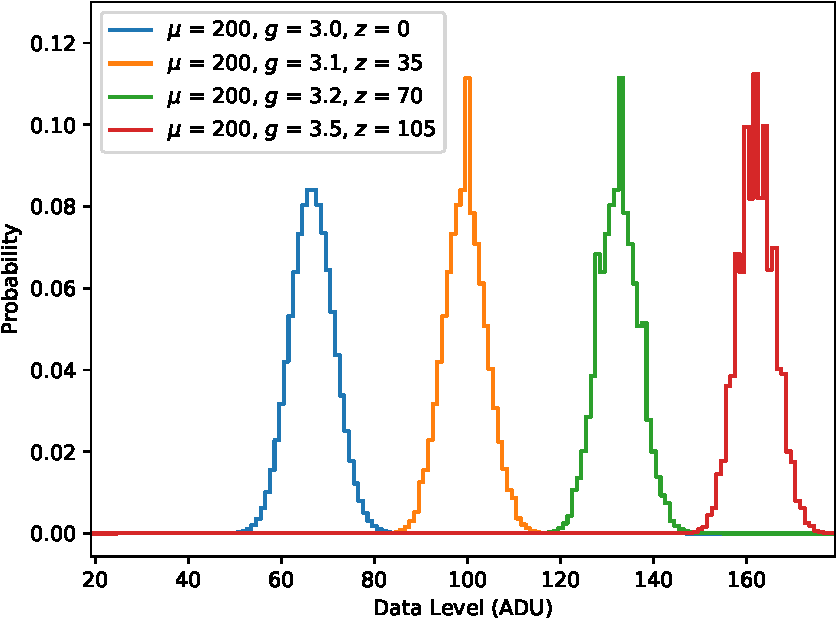
\includegraphics[width=\columnwidth]{figs/histograms}

\caption{Distributions of probabilities of the detector levels for a mean
number of electrons $\mu = 200\,\electron$ and variable gains $g \sim
3\,\electron/\ADU$. The zero-levels $z$ have been chosen to separate the
different distributions. \label{fig:histograms}}
\end{figure}

Assuming $\Round{\ldots}$ rounds to the nearest integer toward zero in the
model~\eqref{eq:ADC-model}, reading the detector value $d$ knowing the actual
number $n_\electron$ of electrons implies that $\omega$ be in a given range:
\begin{equation}
  d - (n_\electron/g) - z - \textfrac12
  ≤ \omega <
  d - (n_\electron/g) - z + \textfrac12 \, .
\end{equation}
Then, provided that the number of electrons $n_\electron$ and the readout noise
$\omega$ be independent and since $n_\electron$ has a Poisson distribution of
parameter $µ$, the probability of the number of ADUs is given by:
\begin{equation}
  \Pr\nolimits_{D}(d)
  = \mathe^{-µ} \, \sum_{n ≥ 0} \frac{µ^n}{n!}
  \int_{d - (n/g) - z + 1/2}^{d - (n/g) - z - 1/2}
  \Pr\nolimits_{\Omega}(\omega)\,\mathd\omega \, ,
\end{equation}
with $\Pr\nolimits_{\Omega}(\omega)$ the probability density function of
$\omega$.  Introducing $\Pr\nolimits_X(x)$ the probability density function
of $x = n_\electron + g\,\omega$ yields:
\begin{equation}
  \Pr\nolimits_{D}(d) = \int_{(d - z + 1/2)\,g}^{(d - z - 1/2)\,g}
  \Pr\nolimits_{X}(x)\,\mathd x \, .
  \label{eq:prob-ADU-exact}
\end{equation}
The distribution $\Pr\nolimits_X(x)$ is a mixture of a Poisson distribution and
of the (scaled) distribution of the readout noise and may thus be a mixture of
Poisson and Gaussian distributions if the readout noise is Gaussian.
Equation~\eqref{eq:prob-ADU-exact} however shows that, whatever the
statistics of the readout noise, $\Pr\nolimits_{D}(d)$ cannot just be the
mixture of Poisson and Gaussian distributions as has been considered by some
authors \citep[\eg,][\etc]{Murtagh_et_all-1995-multiresolution,
Foi_et_al-2008-Poissonian_Gaussian_noise_model_fitting,
Chouzenoux_etal-2015-exact-Poisson_Gaussian_likelihood,
Boulanger_etal-2018-nonsmooth_convex_optimization}.  This is a consequence of
the digitization performed by the ADC.  The effects of digitization can be
illustrated under the simplifying assumption of a negligible readout noise.

In the case of a negligible readout noise ($\omega \approx 0$), reading the
detector value $d$ implies that
the actual number $n_\electron \in \Set{N}$ of electrons is in a given range:
\begin{equation}
  d = \Round*{n_\electron/g + z}
  \quad\Longleftrightarrow\quad
  n_\electron \in \IntRange{n_\Tag{inf}(d,z,g), n_\Tag{sup}(d,z,g)}
\end{equation}
where
\begin{equation}
  \IntRange{a,b} \bydef \Brace*{n \in \Integers \SuchThat a ≤ n ≤ b}\,,
\end{equation}
with $(a,b) \in \Set{Z}^2$, denotes a range of integers and where:
$n_\Tag{inf}(d,z,g)$ and $n_\Tag{sup}(d,z,g)$ are two integer-valued functions
of the number $d$ of ADUs, the zero-level $z$ and the gain $g$:
\begin{align}
   n_\Tag{inf}(d,z,g)
   &= \max\Paren*{0, \Ceil*{\Paren*{d - z - \textfrac12}\,g}}
   \,,\\
   n_\Tag{sup}(d,z,g)
   &= \max\Paren*{0, \Ceil*{\Paren*{d - z + \textfrac12}\,g} -
   1} \,,
\end{align}
with $\Ceil{\ldots}$ the ceiling function. Accounting for the Poisson
distribution of the number $n_\electron$ of electrons, the probability of
getting a value $d$ knowing the mean number $µ$ of electrons, the zero-level
$z$ and the gain $g$ is given by:
\begin{align}
  \Pr\nolimits_{D}(d) = \begin{cases}
   \mathe^{-\mu} \,
   \sum_{n = n_\Tag{inf}(d,z,g)}^{n_\Tag{sup}(d,z,g)}
   \frac{\mu^n}{n!} & \text{$n_\Tag{inf}(d,z,g) ≤ n_\Tag{sup}(d,z,g)$}\\
  0 & \text{else.}
  \end{cases}
  \label{eq:prob-ADU-no-readout-noise}
\end{align}
Figure~\ref{fig:histograms} shows this probability as a function of $d$ for $\mu
= 200\,\electron$ and various gains $g \sim 3\,\electron/\ADU$.

The mean number of levels that yields a given sensor value $d$ is equal to the
gain $g$ but the exact number of levels is given by:
\begin{equation}
  n_\Tag{lev}(d,z,g)
  = \max\Paren[\big]{0, n_\Tag{sup}(d,z,g) - n_\Tag{inf}(d,z,d) + 1}
\end{equation}
which, for given zero-level $z$ and gain $g$, depends on $d$.  Unless the gain
$g$ is integer, the uneven number of electrons that yields a given number of
ADUs leads to irregular distributions (moiré pattern) shown by
Fig.~\ref{fig:histograms}.

Knowing the mean number of electrons $\mu$, the zero-level $z$ and the gain
$g$, the mean and variance of the measured number of ADUs are given by:
\begin{align}
  \Expect*{d}
  &= \sum_d d\,\Pr\nolimits_{D}(d) \, ,
  \label{eq:exact-detector-mean}
  \\
  \Var*{d}
  &= \sum_d \Paren[\big]{d - \Expect*{d}}^2\,
  \Pr\nolimits_{D}(d) \,,
  \label{eq:exact-detector-variance}
\end{align}
where the probability $\Pr\nolimits_{D}(d)$ is given in
Eq.~\eqref{eq:prob-ADU-exact} or Eq.~\eqref{eq:prob-ADU-no-readout-noise}
depending
on whether the readout noise is negligible. Although clipping has been
neglected to simplify this study, there are no closed form expressions for the
above statistical moments.  In what follows, we suggest a simple approximation
of the statistics of the number of ADUs.


\subsection{Approximation of the statistics of the ADUs}

Simple approximations of the expectation and variance of the number of ADUs can
be derived by neglecting the rounding errors due to the digitization:
\begin{align}
  \Expect*{d} &\approx
  \Expect*{n_\electron/g + z + \omega}
  = \mu/g + z \, ,
  \label{eq:detector-mean-with-no-rounding-errors}
   \\
  \Var*{d} &\approx
  \Var*{n_\electron/g + z + \omega} = \mu/g^2 + \sigma^2\, ,
  \label{eq:detector-variance-with-no-rounding-errors}
\end{align}
where $\sigma^2$ is the variance of $\omega$ the readout noise which has been
assumed independent from $n_\electron$ the number of electrons.

Figures~\ref{fig:means} and \ref{fig:variances} plot the differences between
the mean and the variance accounting and not accounting for rounding errors,
that is between Eq.~\eqref{eq:exact-detector-mean} and
Eq.~\eqref{eq:detector-mean-with-no-rounding-errors} for Fig.~\ref{fig:means}
and between Eq.~\eqref{eq:exact-detector-variance} and
Eq.~\eqref{eq:detector-variance-with-no-rounding-errors} for
Fig.~\ref{fig:variances}.  These figures show that there is a small variable
bias $\lesssim 0.005\,\ADU$ for the estimation of the mean given by
Eq.~\eqref{eq:detector-mean-with-no-rounding-errors} while there is almost the
same bias for the variance given by
Eq.~\eqref{eq:detector-variance-with-no-rounding-errors}, except for small
integer gains $g=1$ (the photon-counting case) and $g = 2$ or $3$.  The
variance bias can be approximately estimated assuming that rounding errors are
uniformly distributed on the range $[-\textfrac12,+\textfrac12]$.  Under this
assumption, the variance due to rounding errors has a closed form expression:
\begin{equation}
   \int_{-\textfrac12}^{+\textfrac12}u ^2\,\mathd u = \frac{1}{12}
   \simeq 0.083 \, \ADU^2\, ,
   \label{eq:rounding-errors-variance}
\end{equation}
which is a good approximation of the variance bias in Fig.~\ref{fig:variances},
again except for small integer gains, say $g \in \Brace{1,2,3}$, because
rounding errors are far from being uniformly distributed for such gains.

\begin{figure}
\centering
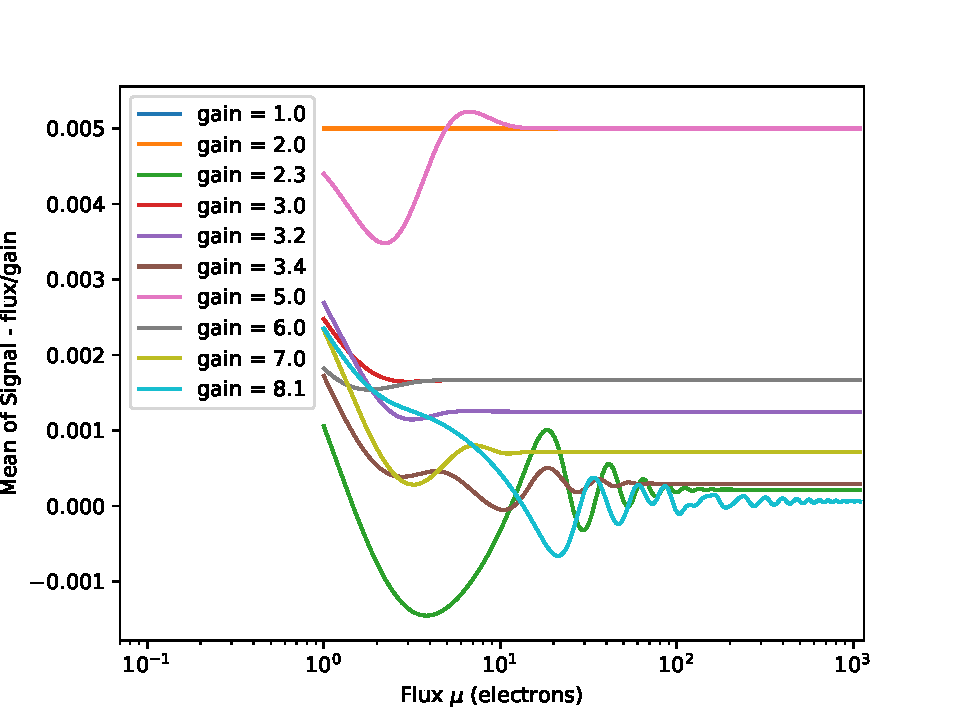
\includegraphics[width=\columnwidth]{figs/means}

\caption{Difference between the mean of the detector signal and $\mu/g$ for
various fluxes $\mu$ and gains $g$.  The curves have been averaged with respect
to the zero-level $z$. \oops{[MT: Where is the curve for gain = 1?]} \oops{[ET:
Vertical axis is in $\ADU$ and tighten margins (for all figs.).]}}
\label{fig:means}
\end{figure}

\begin{figure}
\centering
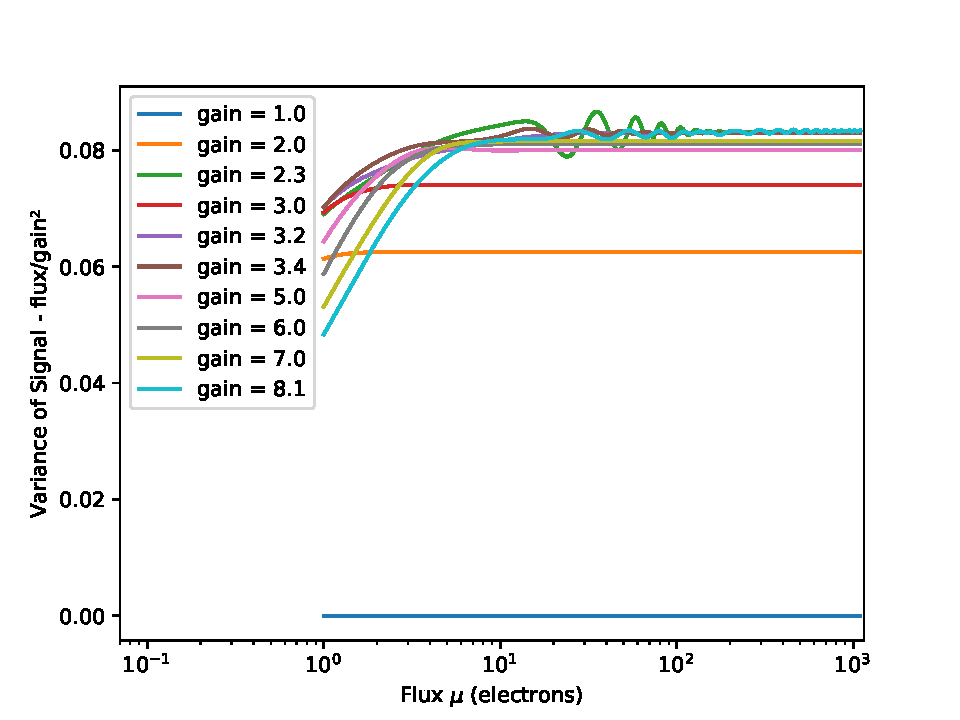
\includegraphics[width=\columnwidth]{figs/variances}

\caption{Difference between the variance of the detector signal and $\mu/g^2$
for various fluxes $\mu$ and gains $g$. The curves have been averaged with
respect to the zero-level $z $. \oops{[ET: Vertical axis is in $\ADU^2$.]}}
\label{fig:variances}
\end{figure}

Using the probability given in Eq.~\eqref{eq:prob-ADU-exact} is not very
convenient and we want to derive more practical approximations of the
distribution of the measured ADUs.  Approximating the sum in
Eq.~\eqref{eq:prob-ADU-no-readout-noise} by the mean number of terms (that is
$g$) times their median value yields:
\begin{align}
  \Pr\nolimits_{D}(d) \approx
  \frac{
    g\,\mathe^{-\mu}\,\mu^{(d - z)\,g}
  }{
    \Gamma\Paren*{(d - z)\,g + 1}
  }
  \label{eq:pdf-ADU-median-approx}
\end{align}
where $\Gamma(x) = \int_0^\infty \mathe^{-t}\,t^{x-1}\,\mathd t$ is the gamma
function.  This expression however also amounts to neglecting the readout
noise. Another possibility is to approximate the distribution of the ADUs in
Eq.~\eqref{eq:prob-ADU-exact} by a Gaussian of mean $\mu/g + z$ and variance
$\mu/g^2 + \sigma^2$ which accounts for the readout noise (and a possible
variance bias) via the term $\sigma^2$.  This approximation yields:
\begin{align}
  \Pr\nolimits_{D}(d)
  \approx \frac{
    \exp\Paren*{
      -\frac{\Paren*{d - \mu/g - z}^2}{2\,\Paren*{\mu/g^2 + \sigma^2}}
    }
  }{
    \sqrt{2\,\pi\,\Paren*{\mu/g^2 + \sigma^2}}
  }\,
  \label{eq:pdf-ADU-Gaussian-approx}
\end{align}
with $\sigma$ the standard deviation of other source of uncertainties than the
shot noise (\eg, the rounding errors and the readout noise). In the case of a
negligible readout noise, the two approximate distributions and the exact one
are shown by Fig.~\ref{fig:pdf-approx} with $\sigma^2 = 1/12$ to account for
rounding errors.  The two approximations appears as good as each other.  The
Gaussian approximation is however easier to handle and has the flexibility to
account for additional sources of noise (e.g., readout noise) via the
parameters $\sigma$ and $z$ (if these other contributions are not centered).

\begin{figure}
\centering
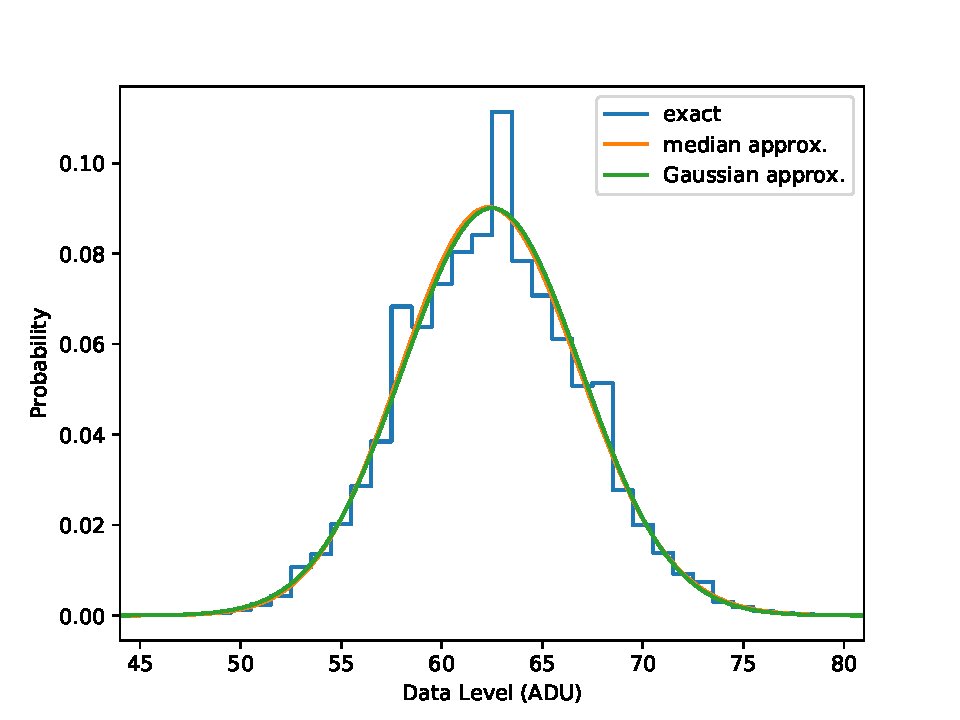
\includegraphics[width=\columnwidth]{figs/pdf-approx}

\caption{Exact distribution of the measured ADUs and its \emph{median} and
Gaussian approximations for a mean number of electrons $\mu = 200$, a gain $g
\sim 3.2$ and a zero-level $z = 0$. The three distributions are respectively
given by Eqs.~\eqref{eq:prob-ADU-no-readout-noise},
\eqref{eq:pdf-ADU-median-approx} and \eqref{eq:pdf-ADU-Gaussian-approx}.}
\label{fig:pdf-approx}
\end{figure}

%An additional source of noise in the measured ADUs is the so-called
%\emph{readout noise}.  The readout noise may be modeled as a random number of
%electrons following a Poissonian distribution with a given mean. In that case,
%the distribution given in Eq.~\eqref{eq:prob-ADU-no-readout-noise} is correct
%provided the mean number of electrons $\mu$ and the zero-level $z$ account for
%this additional contribution. In any case, we will assume the Gaussian
%approximation of the distribution of ADUs in the following. \oops{[ET: Justify
%a bit more and some authors consider that readout is Gaussian.]}

%\oops{Other existing models: Gaussian+Poissonian statistics, Anscombe, etc.
%These distribution may better describe the combination of Poissonian shot
%noise plus some Gaussian readout noise.  However most authors completely
%neglect the effects the analog to digital converter so a simpler approximation
%such as a non homogeneous Gaussian distribution may be easier to deal with
%while providing an approximation just as good as more elaborated ones for
%actual detector data.}


\section{Extracting science data}



\subsection{Accounting for the exposure time and background sources}

Under given observing conditions, the average number of electrons $µ$ and, as a
result, the average number of ADUs scale linearly with the exposure time
$\Delta t$.  This is routinely exploited to calibrate the parameters of the
detector. For the remaining of the paper, it is useful to introduce a
\emph{current} term $c$ which is defined as the number of ADUs delivered per
unit of exposure time:
\begin{equation}
  \label{eq:current}
  c = \frac{µ}{g\,\Delta t} \, ,
\end{equation}
which is expressed in ADU per second ($\ADU/\second$). Replacing $µ$ by
$c\,g\,\Delta t$ in the previous expressions of the expectation and of the
variance of the detector output yields:
\begin{align}
  \Expect{d} &= c\,\Delta t + z\,,\\
  \Var{d} &= c\,\Delta t/g + \sigma^2 \,.
\end{align}
The above expectation shows that $\estim{c} = (d - z)/\Delta t$ is an unbiased
estimator of $c$ given the data $d$.

In practice, the observed object but also some other unwanted sources
contribute to the number of electrons counted by the detector.  To reflect
that, the current term $c$ may be expressed as:
\begin{equation}
  c = c^\Tag{fg} + c^\Tag{bg}
\end{equation}
where the \emph{foreground} term $c^\Tag{fg}$ denotes the contribution of the
source of interest while the \emph{background} term $c^\Tag{bg}$ accounts for
the contribution of all spurious sources.  The detector dark current is part of
the spurious sources which, depending on the wavelength range and on the kind
of observations, may also include the thermal emission of the instrument and
the background emission of the sky.



The scientific exploitation of images acquired by a detector usually requires
to estimate a pixelwise quantity of interest, say $s$, which is proportional to
the light flux received from the observed object.  The quantity of interest is
linearly related to the foreground term $c^\Tag{fg}$

 Due to the ADC gain $g$, to
the quantum efficiency of the detector, to the throughput of the instrument and
perhaps on the transparency of the atmosphere.



 the foreground term $c^\Tag{fg}$ (in $\ADU/\second$) is
not yet the quantity of interest as it depends on the ADC gain $g$ but also on
the quantum efficiency of the detector, on the throughput of the instrument and
perhaps on the transparency of the atmosphere.  All these factors being
potentially different for each detector pixel.


, it is needed
to estimate a pixelwise quantity $s$ which should be proportional to the light
flux received from the observed object.  Owing to the affine relationship
between the expected number of ADUs and the number of electrons...



 be the quantity of interest for the science
Accounting for \emph{background} sources and for the \emph{effective
throughput} ():
\begin{equation}
  c = (s/a) + c^\Tag{bg}
\end{equation}
whit $s$ the quantity of interest for the science (proportional to the mean
number of photons per second received from the object of interest), $a > 0$ a
factor accounting for the instrumental throughput and for the detector quantum
efficiency and $c^\Tag{bg}$ a current term (in $\electron/\ADU$) representing
the contributions of spurious sources such as the sky and instrumental
backgrounds and the detector dark current.

\oops{Calibration data consist in a number of images (detector frames) acquired
under identical conditions (except the exposure time) but different
illumination sources.}


\section{Relevant parameters}

\begin{table}
  \begin{tabular}{ll}
    \hline
    Symbol & Description (Units)\\
    \hline
    \hline
    $a_j$ ($^\ast$) & Conversion factor ($\propto\:$photons/ADU)\\
    $b_j$ & Bias and background correction (ADU)\\
    $c_{j,\ell}$ & Signal rate (ADU/second) \\[0.3ex]
    $c^\Tag{dark}_j$ ($^\ast$) & Dark current (ADU/second) \\[0.3ex]
    $c^\Tag{bg}_{j,\ell}$ & Contribution of spurious background sources\\
    &\multicolumn{1}{l}{(ADU/second)}\\[0.3ex]
    $c^\Tag{fg}_{j,\ell}$ & Contribution of the source(s) of interest\\
    &\multicolumn{1}{l}{(ADU/second)}\\
    $d_{j,k,\ell}$ & Pixel value (ADU) \\
    $e_{j,k,\ell}$ & Noise (ADU) \\
    $g_j$ ($^\ast$) & Gain of analog to digital converter\\
      &\multicolumn{1}{l}{(electrons/ADU)} \\
    $r_{j,\ell}$ & Illumination by the source(s) of interest\\
      &\multicolumn{1}{r}{($\propto\:$photons/second)}\\
    $s_j$ & Signal of interest ($\propto\:$photons) \\
    $\estim{s}_j$ & Estimator of the signal of interest
    ($\propto\:$photons) \\
    $q_j$ & Numerator for the precision of $s_j$ \\
    $r_j$ & Denominator bias for the precision of $s_j$ \\
    $w_j$ & Precision of $s_j$ \\
    $z_j$ ($^\ast$) & Zero-level in analog to digital
    converter (ADU) \\
    $\sigma_j$ ($^\ast$)
    & Standard deviation of the readout noise\\
    & \multicolumn{1}{l}{(ADU/pixel/frame)} \\
    $\Delta t_{k,\ell}$ & Exposure time (seconds) \\
    \hline
  \end{tabular}
  \caption{Notations. Indices $j$ and $k$ are for the pixel and the frame
  respectively. Index $\ell$ specifies the type of illumination. Detector
  parameters, which are common to all data sets, are indicated by an asterisk
  ($^\ast$). ADU stands for \emph{Analog-Digital Units}.  The units of the
  conversion factor $a_j$ and the illumination $r_{j,\ell}$ are given up to a
  factor (denoted by the $\propto$ sign) which is the same for these two
  quantities whatever the pixel, the frame and the type of illumination.}
  \label{tab:notation}
\end{table}


\begin{itemize}
\item the detector  zero-level (or bias) $z$;

\item the detector gain $g$;

\item the detector quantum efficiency;

\item the throughput of the instrument;

\item the standard deviation $\sigma$ of the sources of noise other than shot
noise
\end{itemize}

\subsection{Maximum Likelihood Calibration}


We first consider calibrating the detector parameters and then estimate the
correction of the non-uniformity of the response.  Without loss of generality,
it is easier to first subtract the contribution of the bias and of spurious
background sources to have intermediate data whose expectation is proportional
to the incident flux and to the exposure time. And to second compensate for
the non-uniform throughput and detector gain.

Available calibration data consists in images acquired under various
conditions of illumination and with different (known) exposure times.
For each pixel, the available calibration data is $d_{k,\ell}$ for $(k,\ell)
\in \mathcal{L}$
where index $\ell$ uniquely defines the observing conditions while, for the
\begin{align}
  \Expect{d_{k,\ell}} &= c_{\ell}\,\Delta t_{k,\ell} + z\,,\\
  \Var{d_{k,\ell}} &= c_{\ell}\,\Delta t_{k,\ell}/g + \sigma^2
\end{align}

We first ignore saturations and defective pixels. Assuming independent noise
with a distribution approximately Gaussian, the co-log-likelihood of the data
writes:
\begin{equation}
  \phi(\V\theta) = \sum_{k,\ell}\Paren*{
    \frac{\Paren*{d_{k,\ell} -
        m_{k,\ell}(\V\theta_{\ell})}^2}{v_{k,\ell}(\V\theta_{\ell})}
    + \log\Paren*{v_{k,\ell}(\V\theta_{\ell})}
  }
\end{equation}
with $m_{k,\ell}(\V\theta_{\ell})$ and $v_{k,\ell}(\V\theta_{\ell})$ the
expectation and variance (respectively) of the data $d_{k,\ell}$ knowing the
parameters $\V\theta_{\ell}$ and given by:
\begin{align}
  m_{k,\ell}(\V\theta_{\ell})
  &= c_{\ell}\,\Delta t_{k,\ell} + z \, ,
  \\
  v_{k,\ell}(\V\theta_{\ell})
  &= c_{\ell}\,\Delta t_{k,\ell}/g + \sigma^2 \, ,
\end{align}
for parameters:
\begin{equation}
  \V\theta_{\ell} = \Paren*{z, c_{j,\ell}, g, \sigma} \, .
\end{equation}

\oops{Other possible notation: $m(\V\theta_{\ell}, \Delta t_{k,\ell})$ and
$v(\V\theta_{\ell}, \Delta t_{k,\ell})$.}

The readout noise $\sigma$ accounts for all detector noises, including the
digitization errors.  Hence assuming rounding to the nearest ADU yields
$\sigma ≥ 1/\sqrt{12}$.  Other constraints are $c_{\ell} ≥ 0$ and $g > 0$
because the incident light level and the dark current are nonnegative and the
gain is strictly positive.

In spite of the fact that it is separable in pixels, the maximum likelihood
criterion is not trivial to jointly minimize in all the parameters accounting
for the constraints.  We propose in the following a strategy to solve the
problem and first show how to eliminate the bias and the gain thanks to a
simple change of variables.


\subsubsection{Estimation of the bias and of the gain}

It is convenient to introduce $u = g\,\sigma^2$ so that the variance
writes:
\begin{equation}
  v_{k,\ell}(\V\theta_{\ell}) =
  \Paren*{c_{\ell}\,\Delta t_{k,\ell} + u}/g \,,
\end{equation}
and the maximum likelihood criterion becomes:
\begin{equation}
  \phi(\V\theta) = \sum_{k,\ell}\Paren*{
    g\,\frac{
      \Paren*{d_{k,\ell} - c_{\ell}\,\Delta t_{k,\ell} - z}^2
    }{
      c_{\ell}\,\Delta t_{k,\ell} + u
    }
    + \log\Paren*{c_{\ell}\,\Delta t_{k,\ell} + u} - \log g
  } \,.
\end{equation}
This expression is straightforward to minimize with respect to the bias $z$
leading to the maximum likelihood estimator of the bias knowing the other
parameters. Introducing $\V c = \Paren*{c_{\ell}}_{\ell=1}^L$ with $L$ the
number of considered illuminations, the maximum likelihood estimator of the
bias knowing the other parameters is given by:
\begin{align*}
  z^+(\V c, u)
  &\bydef \argmin_{z} \phi(\V\theta) \notag\\
  &= \argmin_{z} \sum_{k,\ell}\frac{
    \Paren*{d_{k,\ell} - c_{\ell}\,\Delta t_{k,\ell} - z}^2
  }{
    c_{\ell}\,\Delta t_{k,\ell} + u
  }
\end{align*}
which gives:
\begin{equation}
  \boxed{
    z^+(\V c, u) = \frac{
      \sum_{k,\ell}\frac{
        d_{k,\ell} - c_{\ell}\,\Delta t_{k,\ell}
      }{
        c_{\ell}\,\Delta t_{k,\ell} + u
      }
    }{
      \sum_{k,\ell}\frac{1}{c_{\ell}\,\Delta t_{k,\ell} + u}
    }\,.
  }
  \label{eq:best-bias}
\end{equation}
We note that this expression does not depend on the gain $g$ as explicitly
indicated by our notation. Thanks to this independence, the maximum likelihood
estimator of the gain knowing the parameters $\V c$ and $u$ also has a
closed form expression:
\begin{align*}
  g^+(\V c, u)
  &\bydef \argmin_{g} \Brace*{ \min_{\V z} \phi(\V\theta) } \notag\\
  &= \argmin_{g} \sum_{k,\ell} \Paren*{
    g\,\frac{
      \Paren*{
        d_{k,\ell} - c_{\ell}\,\Delta t_{k,\ell} - z^+(\V c, u)
      }^2
    }{
      c_{\ell}\,\Delta t_{k,\ell} + u
    } - \log g
  } \,,
\end{align*}
which gives:
\begin{equation}
  \boxed{
    g^+(\V c, u) = \Avg*{
      \frac{
        \Paren[\big]{
          d_{k,\ell} -c_{\ell}\,\Delta t_{k,\ell} - z^+(\V c, u)
        }^2
      }{
        c_{\ell}\,\Delta t_{k,\ell} + u
      }
    }_{\!\!k,\ell}^{-1}
  }
  \label{eq:best-gain}
\end{equation}
where $\Avg{\ldots}_{k,\ell}$ denotes averaging of the enclosed expression with
respect to indices $k$ and $\ell$. Equations~\eqref{eq:best-bias} and
\eqref{eq:best-gain} show that the remaining parameters to determine are $\V
c$ and $u$ for each pixel.

With the proposed change of variables, $u = g\,\sigma^2$, the constraint on the
readout noise variance becomes $u ≥ g\,\sigma^2_\Tag{min}$ and the standard
deviation of the readout noise in ADU/pixel/frame is given by $\sigma =
\sqrt{u/g}$. Provided the constraints $u > 0$ and $c_{\ell} ≥ 0$ hold, then
$c_{\ell}\,\Delta t_{k,\ell} + u > 0$ and the right hand side of
Eq.~\eqref{eq:best-gain} is strictly positive\footnote{Unless $d_{k,\ell} =
c_{\ell}\,\Delta t_{k,\ell} + z^+(\V c, u)$ whatever $k$ and $\ell$ which
implies exact model and noiseless data!}.

%with:
%\begin{equation}
%  w_{k,\ell}(\V c, u) =
%  1/\Paren*{ c_{\ell}\,\Delta t_{k,\ell} + u} \, ,
%\end{equation}
%the precision of the datum $d_{k,\ell}$ divided by the gain $g$.

\subsubsection{Separable estimation of the other parameters}

\oops{Due to the assumed independent statistics, the co-log-likelihood is
separable with respect to the pixel index $j$.}

We have just shown that $\phi(\V\theta)$ can be jointly minimized in $z$ and
$g$ so the problem reduces to:
\begin{align}
  \Paren[\big]{\estim{\V c}, \estim{u}}
  &= \argmin_{\V c ≥ 0, u > 0}
  \Brace[\Big]{\min_{g,z} \phi(\V\theta)} \notag \\
  &= \argmin_{\V c ≥ 0, u > 0} \psi(\V c, u)
\end{align}
with:
\begin{align}
  \psi(\V c, u)
  &= g^+(\V c, u)\,\sum_{k,\ell} \frac{
    \Paren*{d_{k,\ell} - c_{\ell}\,\Delta t_{k,\ell} - z^+(\V c, u)}^2
  }{
    c_{\ell}\,\Delta t_{k,\ell} + u
  } \notag\\
  &\quad + \sum_{k,\ell}\log\Paren*{c_{\ell}\,\Delta t_{k,\ell} + u}
  - n\,\log g^+(\V c, u) \,,
\end{align}
with \oops{$n$} the number of terms in $\sum_{k,\ell}$.

\paragraph{Non-linear optimization} There is no closed form for the minimum of
$\psi(\V c, u)$, but starting from some initial guess $\V c\Iter0$ and
$u\Iter0$, $\psi(\V c, u)$ can be minimized by a nonlinear multi-dimensional
optimization algorithm implementing bound constraints, \eg BOBYQA
\citep{Powell-2009-BOBYQA} or VMLMB \citep{Thiebaut-2002-optim_bdec}. To
simplify the equations, we introduce the \emph{residuals} and the precision
(divided by the gain):
\begin{align}
  x_{k,\ell}(\V c, u)
  &= d_{k,\ell} - c_{\ell}\,\Delta t_{k,\ell} - z^+(\V c, u) \,, \\
  w_{k,\ell}(\V c, u)
  &= \Paren*{c_{\ell}\,\Delta t_{k,\ell} + u}^{-1}\,,
\end{align}
so that:
\begin{equation}
  \psi(\V c, u) = \sum_{k,\ell} \Paren*{
    g^+\,w_{k,\ell}\,x_{k,\ell}^2 - \log g^+ - \log w_{k,\ell}
 } \, ,
\end{equation}
where the dependency of all the terms of the right hand side with $\V c$ and
$u$ is implicitly assumed to simplify the expression. The partial derivatives
of the criterion are needed by VMLMB. These derivatives are given by:
\begin{align}
  \PDer{\psi(\V c, u)}{c_{\ell}}
  &=\sum_{k} w_{k,\ell}\cdot\Paren*{
    1 - g^+ \cdot x_{k,\ell}\cdot\Paren*{2 + w_{k,\ell}\cdot x_{k,\ell}}
  }\cdot\Delta t_{k,\ell} \,,\\
  \PDer{\psi(\V c, u)}{u}
  &= \sum_{k,\ell} w_{k,\ell}\cdot\Paren*{
    1 - g^+ \cdot w_{k,\ell} \cdot x_{k,\ell}^2
  } \,.
\end{align}
To obtain these expressions one has to account for the fact that $z^+(\V c,
u)$ and $g^+(\V c, u)$ minimize $\phi(\V\theta)$ in $z$ and $g$.

To speedup iterations, a diagonal preconditioner can be implemented using the
following approximations for the second derivatives:
\begin{align}
  \PDer{^2\psi(\V c, u)}{c_{\ell}^2}
  &= 2\,g^+\,\sum_{k} w_{k,\ell}\,
    \Paren*{1 + w_{k,\ell}\,x_{k,\ell}}^2\,\Delta t_{k,\ell}^2
    - \sum_{k} w_{k,\ell}^2\,\Delta t_{k,\ell}^2
  \notag\\
  &\quad - \PDer{g^+}{c_\ell}\,\sum_{k} w_{k,\ell}\,x_{k,\ell}\,
  \Paren*{2 + w_{k,\ell}\,x_{k,\ell}}\,\Delta t_{k,\ell}
  \notag\\
  &\quad + 2\,g^+\,\sum_{k} w_{k,\ell}\,\Paren*{
    1 + w_{k,\ell}\,x_{k,\ell}
  }\,\Delta t_{k,\ell}\,\PDer{z^+}{c_\ell}
  \notag\\
  &\oops{
    \approx \sum_{k} w_{k,\ell}\,\Paren*{2\,g^+ + w_{k,\ell}}
    \,\Delta t_{k,\ell}^2
  } \,,\\
  %
  \PDer{^2\psi(\V c, u)}{u^2}
  &= 2\,g^+\,\sum_{k,\ell} w_{k,\ell}^3\,x_{k,\ell}^2
   - \sum_{k,\ell} w_{k,\ell}^2
  \notag\\
  &\quad - \PDer{g^+}{u}\,\sum_{k,\ell} w_{k,\ell}^2\,x_{k,\ell}^2
  \notag\\
  &\quad+ 2\,g^+\,\sum_{k,\ell} w_{k,\ell}^2\,x_{k,\ell}\,\PDer{z^+}{u}
  \notag\\
  &\oops{\approx \sum_{k,\ell} w_{k,\ell}^2} \,,
\end{align}
where the two approximations follows from the following approximate and exact
averaged values:
\begin{align*}
  \Avg[\big]{w_{k,\ell}(\V c, u)\,x_{k,\ell}(\V c, u)}_{k}
  &\approx 0 \,,\\
  g^+(\V c, u)\,\Avg[\big]{w_{k,\ell}(\V c, u)\,
    x_{\ell}^2(\V c, u)}_{k,\ell}
  &= 1\,,
\end{align*}
the latter is a direct consequence of Eq.~\eqref{eq:best-gain}.

%We therefore drop the pixel index $j$ in what follows for the sake of
%simplicity and attempt to solve:
%\begin{equation}
%  \estim{\V\theta} = \argmin_{\V\theta \in \Omega} \Brace*{
%    \varphi(\V\theta) = \sum_{k,\ell}\Paren*{
%      \frac{\Paren*{d_{k,\ell} -
%m_{k,\ell}(\V\theta)}^2}{v_{k,\ell}(\V\theta)}
%      + \log\Paren*{v_{k,\ell}(\V\theta)}
%    }
%  }
%\end{equation}
%with, using the parameter $u$ instead of $\sigma$, $\V\theta =
%(b,\Paren*{c_{\ell}}_{\ell=1,2,\ldots},g,u)$, $\Omega$ the feasible set of
%acceptable parameters and:
%\begin{align}
%  m_{k,\ell}(\V\theta)
%  &= c_{\ell}\,\Delta t_{k,\ell} + z \, ,
%  \\
%  v_{k,\ell}(\V\theta)
%  &= \Paren*{c_{\ell}\,\Delta t_{k,\ell} + u}/g \,.
%\end{align}
%The feasible set $\Omega$ accounts for constraints on the parameters:
%\begin{equation}
%  \Omega = \Brace*{
%    \V\theta = (b,\Paren*{c_{\ell}}_{\ell=1,2,\ldots},g,u) \in
%    \Reals^{3+n_\Tag{cls}} \SuchThat
%    \forall\ell, c_\ell ≥ 0, g > 0, u ≥ g/12
%  } \, .
%\end{equation}

\oops{Another possibility would be to use an Iterative Reweighted Least Squares
(IRLS) method.}

\paragraph{Initial solution} Whatever the chosen non-linear optimization
method, the problem being non-convex, providing a starting point not too far
from the solution is of prime importance. We note that if the zero-level $z$
and the ratio $\tau_{\ell} = u/c_{\ell} > 0$ are assumed known, the
\emph{current} terms $c_{\ell}$ are approximately solutions of simple
independent linear least squares problems:
\begin{align}
  c^+_{\ell}(z,\tau)
  &= \argmin_{{\ell}}\phi(\V\theta)
  \quad\text{s.t.\ $u = \tau\,c_{\ell}$}\quad \notag\\
  &\approx \argmin_{c ≥ 0}\sum_{k} \frac{
    \Paren*{d_{k,\ell} - c\,\Delta t_{k,\ell} -  z}^2
  }{
    \Delta t_{k,\ell} + \tau
  } \notag\\
  &\approx \max\Brace*{0, \frac{
    \sum_{k} \frac{
      \Paren*{d_{k,\ell} - z}\,\Delta t_{k,\ell}
    }{
      \Delta t_{k,\ell} + \tau
    }
  }{
    \sum_{k} \frac{\Delta t_{k,\ell}^2}{\Delta t_{k,\ell} + \tau}
  }} \,.
  \label{eq:simple-c}
\end{align}
In practice, we choose the initial estimation of the zero-level for the
considered pixel to be the least value taken by this pixel for all frames:
\begin{equation}
  z\Iter0 = \min_{k,\ell} d_{k,\ell} \,.
  \label{eq:initial-bias}
\end{equation}
We further impose that $\tau_{\ell} = \tau$ be the same for all kinds
of illuminations $\ell$ and for all pixels $j$ and negligible compared to all
non-zero exposure times:
\begin{equation}
  \tau = \varepsilon_1\,
  \min_{\substack{
      k,\ell\\
      \Delta t_{k,\ell} > 0
  }} \Delta t_{k,\ell} \,,
  \label{eq:tau}
\end{equation}
where  $\varepsilon_1 > 0$ is a small factor, and then choose the initial
\emph{current} terms according to Eq.~\eqref{eq:simple-c}:
\begin{equation}
  c\Iter0_{\ell} %= c^+_{\ell}\Paren[\big]{z\Iter0,\tau}
  = \frac{
    \sum_{k} \frac{
      \Paren*{d_{k,\ell} - z\Iter0}\,\Delta t_{k,\ell}
    }{
      \Delta t_{k,\ell} + \tau
    }
  }{
    \sum_{k} \frac{\Delta t_{k,\ell}^2}{\Delta t_{k,\ell} + \tau}
  }\,.
  \label{eq:initial-c}
\end{equation}
To select the initial value $u\Iter0$ of $u$, we assume that the readout
noise is small for most cases and take the initial value to be the least
nonzero value of $c_{\ell}\Iter0\,\Delta t_{k,\ell}$ times a small factor
$\varepsilon_2 > 0$:
\begin{equation}
  u\Iter0 = \varepsilon_2 \,
  \min_{\substack{
      k,\ell\\
      c_{\ell}\Iter0\,\Delta t_{k,\ell} > 0
  }} c_{\ell}\Iter0\,\Delta t_{k,\ell} \,.
  \label{eq:initial-u}
\end{equation}
This choice ensures that $u\Iter0 > 0$.  Finally the initial estimate of the
pixelwise gain is given by Eq.~\eqref{eq:best-gain} but using the initial bias
instead of the best bias given $\V c\Iter0$ and $u\Iter0$:
\begin{equation}
  g\Iter0 = \Avg*{
    \frac{
      \Paren[\big]{
        d_{k,\ell} -c\Iter0_{\ell}\,\Delta t_{k,\ell} - z\Iter0
      }^2
    }{
      c\Iter0_{\ell}\,\Delta t_{k,\ell} + u\Iter0
    }
  }_{\!\!k,\ell}^{-1} \, .
  \label{eq:initial-gain}
\end{equation}
Thus the initial solution is determined by the choice of two small positive
constants.  In practice, we take $\varepsilon_1 = \varepsilon_2 = 1/10$.

% Bibliography.
\bibliographystyle{aa}
\bibliography{calibration-of-scientific-detectors}

\end{document}
